\documentclass[stu, 12pt, letterpaper, donotrepeattitle, floatsintext, natbib]{apa7}
%\usepackage[utf8]{inputenc}
\usepackage{fontspec} %paquete para usar la fuente Arial 12
\usepackage{comment}
\usepackage{marvosym}
\usepackage{graphicx}
\usepackage{float}
\usepackage{fancyhdr}
\usepackage[normalem]{ulem}
\usepackage[spanish]{babel} 
\usepackage{lastpage} %para le formato que quiere la profe QUITAR SI QUIERES OG APA7
\usepackage{ragged2e} %para le formato que quiere la profe QUITAR SI QUIERES OG APA7
\usepackage{indentfirst} %para le formato que quiere la profe QUITAR SI QUIERES OG APA7

%comando para ajustar la fuente Arial en todo el documento
\setmainfont{Arial} %COMPILAR DOC CON XeLateX DOS VECES

\DeclareCaptionLabelSeparator*{spaced}{\\[2ex]}
%\captionsetup[table]{textfont=it,format=plain,justification=justified,
% singlelinecheck=false,labelsep=spaced,skip=1pt}

\selectlanguage{spanish}

\useunder{\uline}{\ul}{}
\newcommand{\myparagraph}[1]{\paragraph{#1}\mbox{}\\}


\rfoot{\thepage}%QUITAR SI QUIERES OG APA7 
\rhead{} %QUITAR SI QUIERES OG APA7
%\setcounter{secnumdepth}{3} %permite enumerar las secciones QUITAR SI QUIERES OG APA7
\setlength{\parindent}{1.27cm} %sangria forzada QUITAR SI QUIERES OG APA7

\renewcommand\labelitemi{$\bullet$}

\newcommand*\chem[1]{\ensuremath{\mathrm{#1}}}

\fancypagestyle{portada}
{
    \fancyhf{}
    \chead{
\includegraphics[width=16cm]{logosITT.png}}
}

\begin{document}
    %PORTADA
    \begin{titlepage}
        \thispagestyle{portada}
        \centering
        \vspace*{0.2cm}
        {\large\scshape\bfseries Tecnológico Nacional de México\\Instituto Tecnológico de Tijuana\par}
        \vspace{0.6cm}
        {\normalsize\scshape\bfseries Subdirección Académica\\Departamento de Sistemas y Computación\par}
        \vspace{0.6cm}
        {{\bfseries SEMESTRE:}\\Enero - Junio 2022\par}
        \vspace{\baselineskip}
        {{\bfseries CARRERA:}\\Ing. Sistemas Computacionales\par}
        \vspace{\baselineskip}
        {{\bfseries MATERIA:}\\SCB-1001SC6C Administración de Bases de Datos\par}
        \vspace{\baselineskip}
        {{\bfseries TITULO ACTIVIDAD:}\\Portafolio de evidencias\par}
        \vspace{\baselineskip}
        {{\bfseries UNIDAD A EVALUAR:}\\Unidad 2 \par}
        \vspace{\baselineskip}
        {{\bfseries NOMBRE Y NUMERO DE CONTROL DEL ALUMNO:}\\Abraham Jhared Flores Azcona, 19211640\par}
        \vspace{\baselineskip}
        {{\bfseries NOMBRE DEL MAESTRO(A):}\\M.A. Gabriela Lourdes Tapia Gonzales\par}
        \vspace{\baselineskip}
    \end{titlepage}

% Índices
\pagenumbering{arabic}
    % Contenido
\renewcommand\contentsname{Contenido}
\tableofcontents
\pagebreak
% Cuerpo 
    %NOTA: PARA CITAR ESTILO "Merts (2003)" usar \cite{<nombre_cita_bib>}
    %                        "(Metz, 1978)" usar \citep{<nombre_cita_bib>}
\section{Introducción}
    \begin{justifying}
Como parte de los requisitos de la materia, se necesita realizar un compendio de pruebas
de las actividades realizadas por el alumno y dar a entender que cumplió con los deberes encargados y tener derecho a realizar el examen 
correspondiente a la unidad a evaluar. En este portafolio se recolectan las actividades realizadas a lo largo de la unidad, que en su mayoría
consistieron en aprender y manejar ciertos aspectos de los SGBD.\par
    \end{justifying}
\vspace{\baselineskip}
\section{Arquitectura e instalación de SGBD}
    \begin{figure}[H]
        \caption{\emph{Captura de pantalla de la actividad de laboratorio 1\\}}
        \centering
        \smallskip
        
\includegraphics[width=17cm, height=10cm]{act1.jpg}
        \bigskip
        \justifying\small\textit{Nota}. %\cite{tomta-2009}. %citar al tmta. 
        Autoría Propia (2022).
\end{figure}
\vspace{\baselineskip}
\section{Práctica 1: instalación de instancia}
\begin{figure}[H]
    \caption{\emph{Captura de pantalla de la práctica 1\\}}
    \centering
    \smallskip
    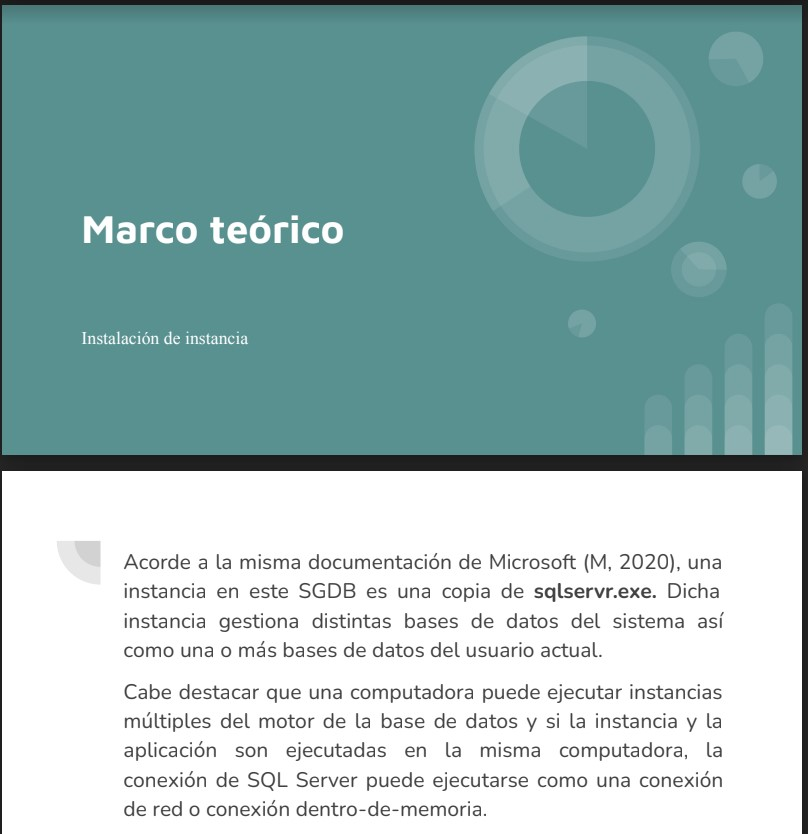
\includegraphics[width=17cm, height=12cm]{act2.jpg}
    \bigskip
    \justifying\small\textit{Nota}. %\cite{tomta-2009}. %citar al tmta. 
    Autoría Propia (2022).
\end{figure}
\vspace{\baselineskip}
\section{Práctica 2: Servicios de arranque y paro de servicios}
\begin{figure}[H]
    \caption{\emph{Captura de pantalla de la práctica 2\\}}
    \centering
    \smallskip
    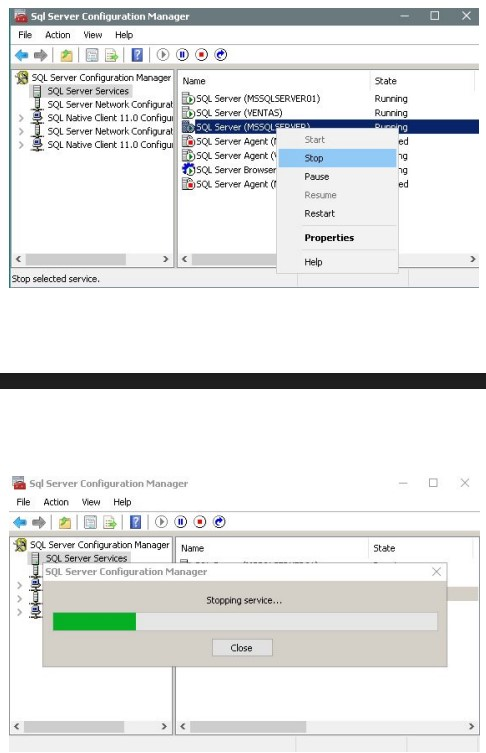
\includegraphics[width=17cm, height=12cm]{act3.jpg}
    \bigskip
    \justifying\small\textit{Nota}. %\cite{tomta-2009}. %citar al tmta. 
    Autoría Propia (2022).
\end{figure}
\vspace{\baselineskip}
\section{Práctica 3: Configuración de servicios}
\begin{figure}[H]
    \caption{\emph{Captura de pantalla de la práctica 3\\}}
    \centering
    \smallskip
    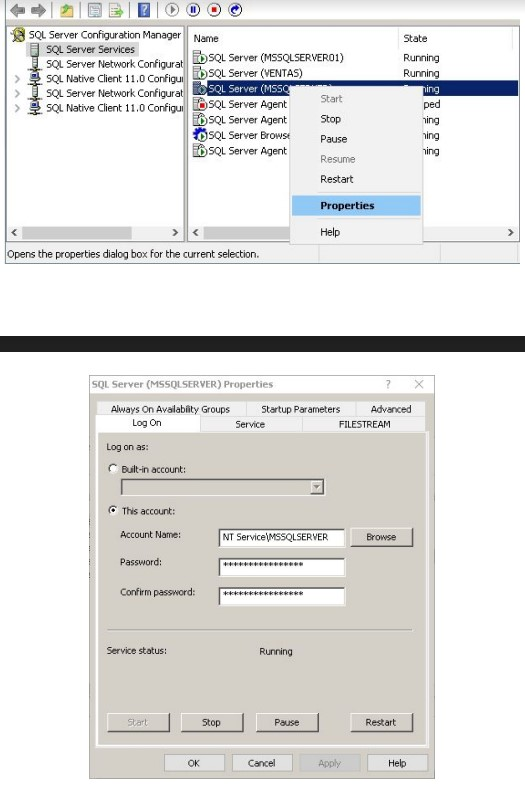
\includegraphics[width=17cm, height=12cm]{act4.jpg}
    \bigskip
    \justifying\small\textit{Nota}. %\cite{tomta-2009}. %citar al tmta. 
    Autoría Propia (2022).
\end{figure}
\vspace{\baselineskip}
\section{Caso de estudio: Requisitos del sistema de AutoCAD 2021/2022 including Specialized Toolsets}
\begin{figure}[H]
    \caption{\emph{Captura de pantalla del caso de estudio\\}}
    \centering
    \smallskip
    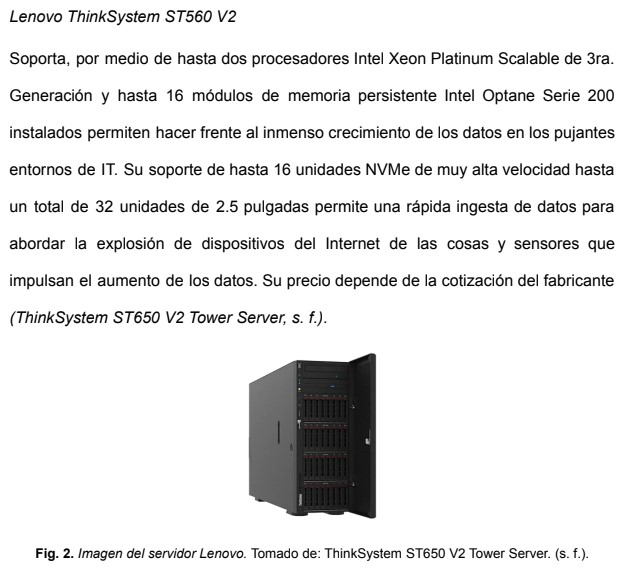
\includegraphics[width=17cm, height=12cm]{caso.jpg}
    \bigskip
    \justifying\small\textit{Nota}. %\cite{tomta-2009}. %citar al tmta. 
    Autoría Propia (2022).
\end{figure}
\vspace{\baselineskip}
\section{Examen de evaluación unidad 2}
\begin{figure}[H]
    \caption{\emph{Captura de pantalla del examen\\}}
    \centering
    \smallskip
    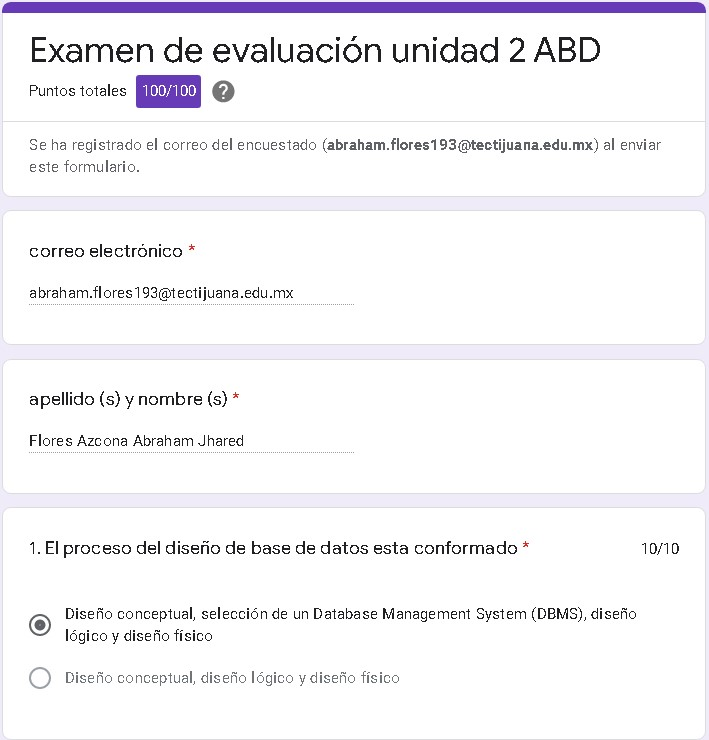
\includegraphics[width=17cm, height=12cm]{test.jpg}
    \bigskip
    \justifying\small\textit{Nota}. %\cite{tomta-2009}. %citar al tmta. 
    Autoría Propia (2022).
\end{figure}

\section{Conclusión}
    \begin{justifying}
El realizar este compendio de actividades permite recordar qué se ha hecho hasta el momento, que nos permite reflexionar sobre nuestro avance.
Debido a que esta unidad ha sido más práctica que la anterior, es recomendable repasar lo aprendido para mejorar la destreza de lo efectuado.\par
    \end{justifying}
\end{document}